% Unofficial BGU Poster template.
% A fork of the UCPH Template https://www.overleaf.com/latex/templates/ucph-poster-template/kgxvdxjbrtpf
% which is a fork of the UMich template https://www.overleaf.com/latex/templates/university-of-michigan-umich-poster-template/xpnqzzxwbjzc
% which is a fork of the MSU template https://www.overleaf.com/latex/templates/an-unofficial-poster-template-for-michigan-state-university/wnymbgpxnnwd
% which is a fork of https://www.overleaf.com/latex/templates/an-unofficial-poster-template-for-new-york-university/krgqtqmzdqhg
% which is a fork of https://github.com/anishathalye/gemini
% also refer to https://github.com/k4rtik/uchicago-poster

\documentclass[final]{beamer}

% ====================
% Packages
% ====================

\usepackage[T1]{fontenc}
 \usepackage[utf8]{luainputenc}
\usepackage{lmodern}
\usepackage[size=custom, width=48,height=48, scale=0.6]{beamerposter}
\usetheme{gemini}
\usecolortheme{bgu}
\usepackage{graphicx}
\usepackage{booktabs}
\usepackage{tikz}
\usepackage{pgfplots}
\pgfplotsset{compat=1.14}
\usepackage{anyfontsize}
\usepackage{caption}
\usepackage{subcaption}

% ====================
% Lengths
% ====================

% If you have N columns, choose \sepwidth and \colwidth such that
% (N+1)*\sepwidth + N*\colwidth = \paperwidth
\newlength{\sepwidth}
\newlength{\colwidth}
\setlength{\sepwidth}{0.025\paperwidth}
\setlength{\colwidth}{0.3\paperwidth}

\newcommand{\separatorcolumn}{\begin{column}{\sepwidth}\end{column}}

% ====================
% Title
% ====================

\title{PETIT-GAN: Physically Enhanced Thermal Image-Translating Generative Adversarial Network}

\author{Omri Berman, Navot Oz, David Mendlovic, Nir Sochen, Yafit Cohen, Iftach Klapp}

\institute[shortinst]{Tel Aviv University, Tel Aviv, Israel \\Agricultural Research Organization - Volcani Institute, Rishon LeZion, Israel}
% \institute[shortinst]{}

% ====================
% Footer (optional)
% ====================

\footercontent{
  \href{https://github.com/bermanz/PETIT}{\textbf{Project Website: https://github.com/bermanz/PETIT}} \hfill
  \href{omriberman@mail.tau.ac.il}{\textbf{Contact: omriberman@mail.tau.ac.il}}}
% (can be left out to remove footer)

% ====================
% Logo (optional)
% ====================

% use this to include logos on the left and/or right side of the header:
% Left: institution
\logoright{
\includegraphics[height=5cm]{../figs/logos/volcani_big.png}}
\logoleft{
\includegraphics[width=5cm]{../figs/logos/TAU_logo.png}}
% Right: funding agencies and other affilations 
%\logoright{\includegraphics[height=7cm]{logos/NSF.eps}}
% ====================
% Body
% ====================

\begin{document}



\begin{frame}[t]
\begin{columns}[t]
\separatorcolumn

% --------------------- 1st column ---------------------

\begin{column}{\colwidth}

  \begin{block}{Introduction}
    Thermal multispectral imagery is imperative for a plethora of environmental applications.
    Unfortunately, there are no publicly-available datasets of thermal multispectral images with a high spatial resolution that would enable the development of algorithms and systems in this field.    
    To tackle this issue, we combined a physically modeled prior information an unpaired image-to-image (UI2I) translation model to produce synthetic multispectral thermal images.
    Our contributions are:
    \begin{itemize}
      \item Introduction of a novel thermal aerial images dataset with unpaired images of different spectral bands.
      \item Application of UI2I between different thermal image modalities;
      \item Development and utilization of an analytic-physical-UI2I translation model;
    \end{itemize}                
  \end{block}

  \begin{block}{Thermal Aerial Multispectral Dataset}

    We collected the multispectral data for training our model using a lightweight airplane, 2000 meters above ground.
    The plane conducted several flights, each with some IR filter (monochromatic) or without (panchromatic).
    \begin{figure}
      \centering
      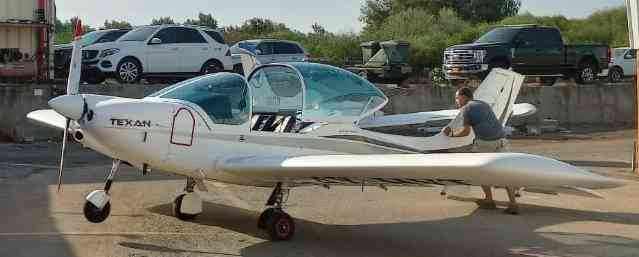
\includegraphics[width=\textwidth]{../figs/data/light_airplane.jpeg}
      % \caption{Lightweight airplane used for the data collection}
    \end{figure}
    Due to the nature of flight conditions, data collected for each channel is inherently unpaired to the others, which led us toward developing an UI2I solution.    
  \end{block}

  \begin{exampleblock}{Mathematical background}
    \begin{itemize}
      \item \emph{Blackbody Radiation}: electromagnetic emission of an ideal opaque object due to its temperature, described by the Stephan-Boltzmann equation:
            \begin{equation*} \label{eq:stephan-boltzmann-ideal}
                P(T) = \int_0^\infty \frac{2\pi hc^2}{\lambda^5}\frac{1}{e^{\frac{hc}{\lambda kT}} - 1} d\lambda = \frac{\sigma}{\pi} T^4 \; \; \left[W sr^{-1} m^{-2}\right]
            \end{equation*}
            % \begin{figure}
            %   \centering
            %   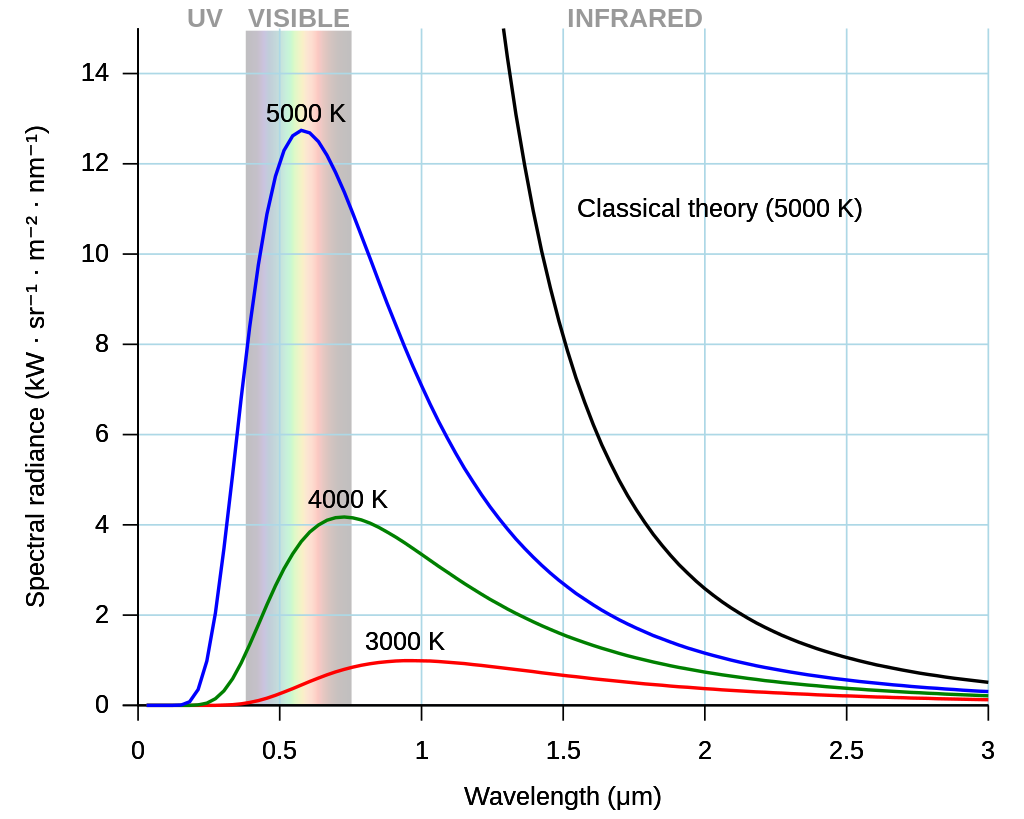
\includegraphics[width=0.3\linewidth]{../figs/methods/planck.png}
            % \end{figure}
      \item In practical thermal imaging, the image intensity depends on the both the object's temperature ($T_\mathit{obj}$) and the camera's intrinsic temperature ($T_\mathit{int}$). 
            Nugent et al. \cite{10.1117/1.OE.52.6.061304} suggested 3rd order polynomials for the dependency in the ambient temperature:
            \begin{equation*} \label{eq:IntensityVsTemperatures}
              \begin{split}            
                I(T_\mathit{obj}, T_\mathit{int}) &= p^{(0)}_c(T_\mathit{int}) T^4_\mathit{obj} + p^{(1)}_c(T_\mathit{int})\\
                p^{(i)}_c(T_\mathit{int}) &= \sum_{k=0}^3  c_{i,k} T_\mathit{int}^k
            \end{split}
            \end{equation*}
    \end{itemize}
  \end{exampleblock}

\end{column}

\separatorcolumn

% --------------------- 2nd column ---------------------
\begin{column}{\colwidth}

  \begin{alertblock}{Method}

    \begin{itemize} 
      \item \textbf{Physical UI2I model}\linebreak\linebreak
        We rely on Nugent et al.'s theorem to calibrate 2 physical polynomial transformations:
        \begin{itemize}
          \item Transformation of panchromatic intensities to object temperatures:
          \begin{equation*}
            \hat{T}_\mathit{obj} = \sqrt[\leftroot{5} 4]{\frac{\pmb{I_\mathit{pan}} - p^{(0)}_{c_\mathit{pan}}(\pmb{T_\mathit{pan}})}{p^{(1)}_{c_\mathit{pan}}(\pmb{T_\mathit{pan}})}}
          \end{equation*}
          \item Transformation of object temperatures to monochromatic intensities.
          \begin{equation*}
            \hat{I}_\mathit{mono} = p^{(1)}_{c_\mathit{mono}}(\pmb{T_\mathit{mono}}) \pmb{\hat{T}_\mathit{obj}}^4 + p^{(0)}_{c_\mathit{mono}}(\pmb{T_\mathit{mono}})
          \end{equation*}
        \end{itemize}

        The two transformations are cascaded to get a complete panchromatic to monochromatic UI2I model.
        \begin{figure}
            \centering
            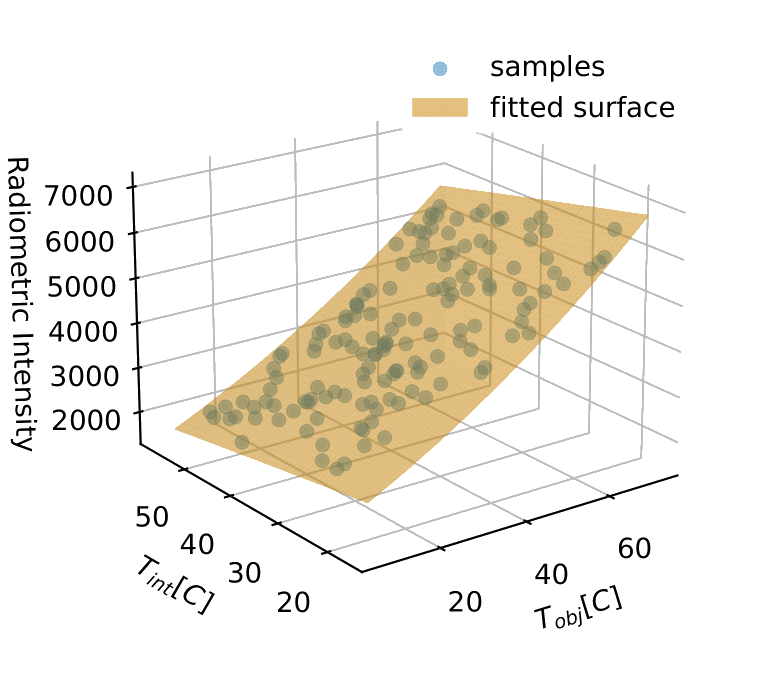
\includegraphics[width=0.5\textwidth]{../figs/methods/physical_model_tight.png}
            % \caption{Calibrated model coefficients Illustration}
        \end{figure}
    
      % To calibrate the polynomials coefficients, we designed a dedicated calibration setup, including a thermal camera, an environmental chamber, and a blackbody target.
      % \begin{figure}
      %   \centering
      %   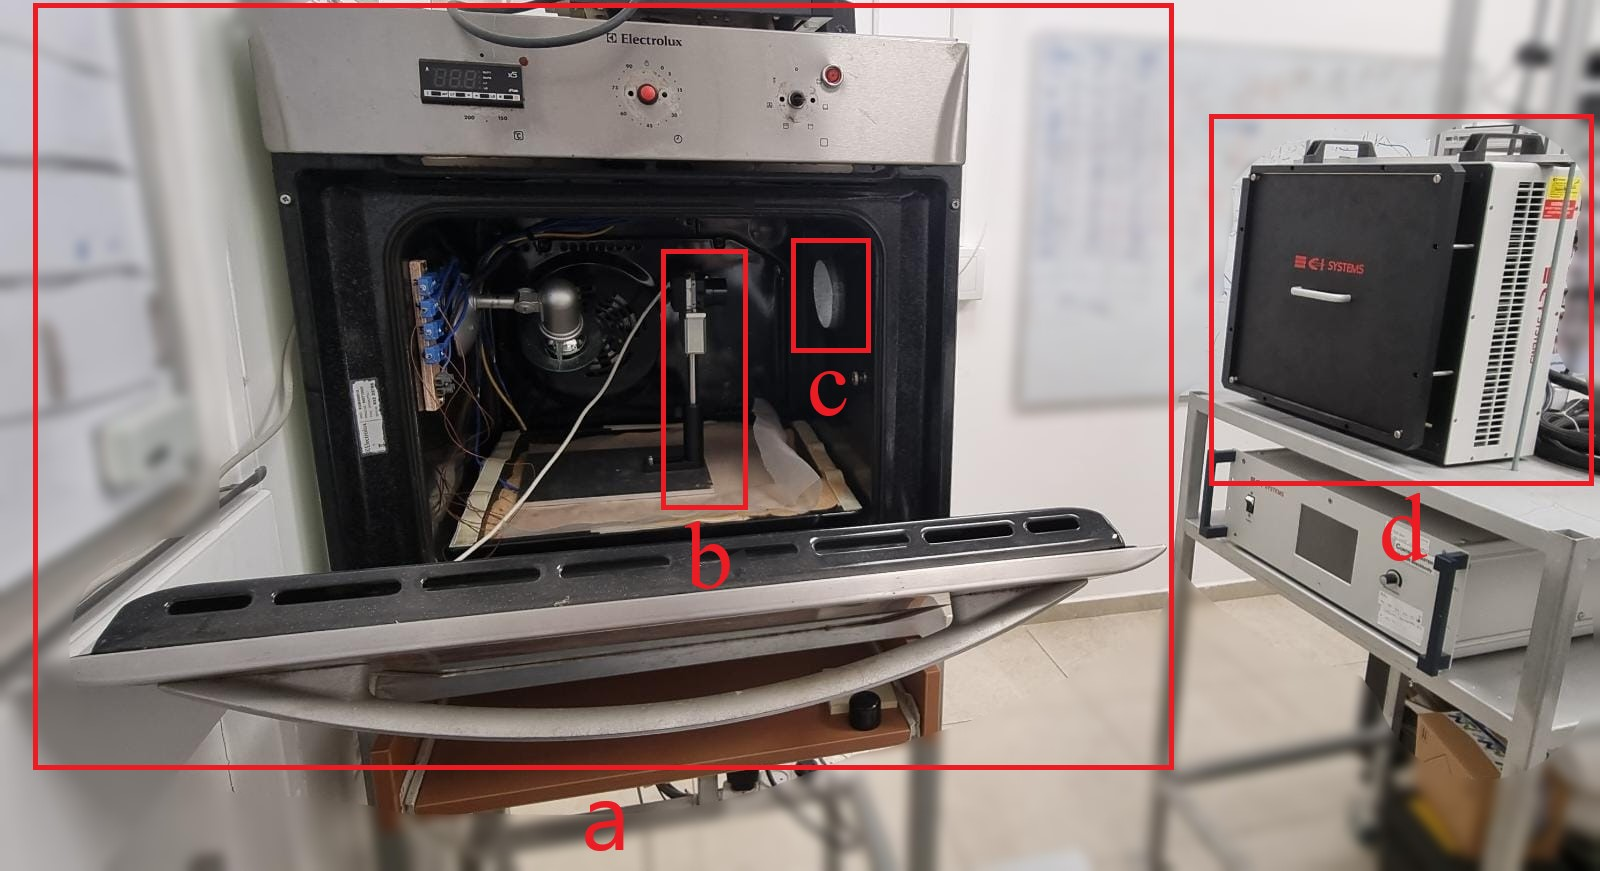
\includegraphics[width=0.9\textwidth]{../figs/methods/calib_setup.jpg}
      %   \caption{Calibration setup}
      % \end{figure}    
      \item \textbf{PETIT}\linebreak\linebreak
        Our physical UI2I model is fused with a deep generative adversarial network (GAN) generator, who's architecture is based on those of CycleGAN \cite{CycleGAN2017} and CUT \cite{park2020cut}.
        \begin{figure}
          \centering
          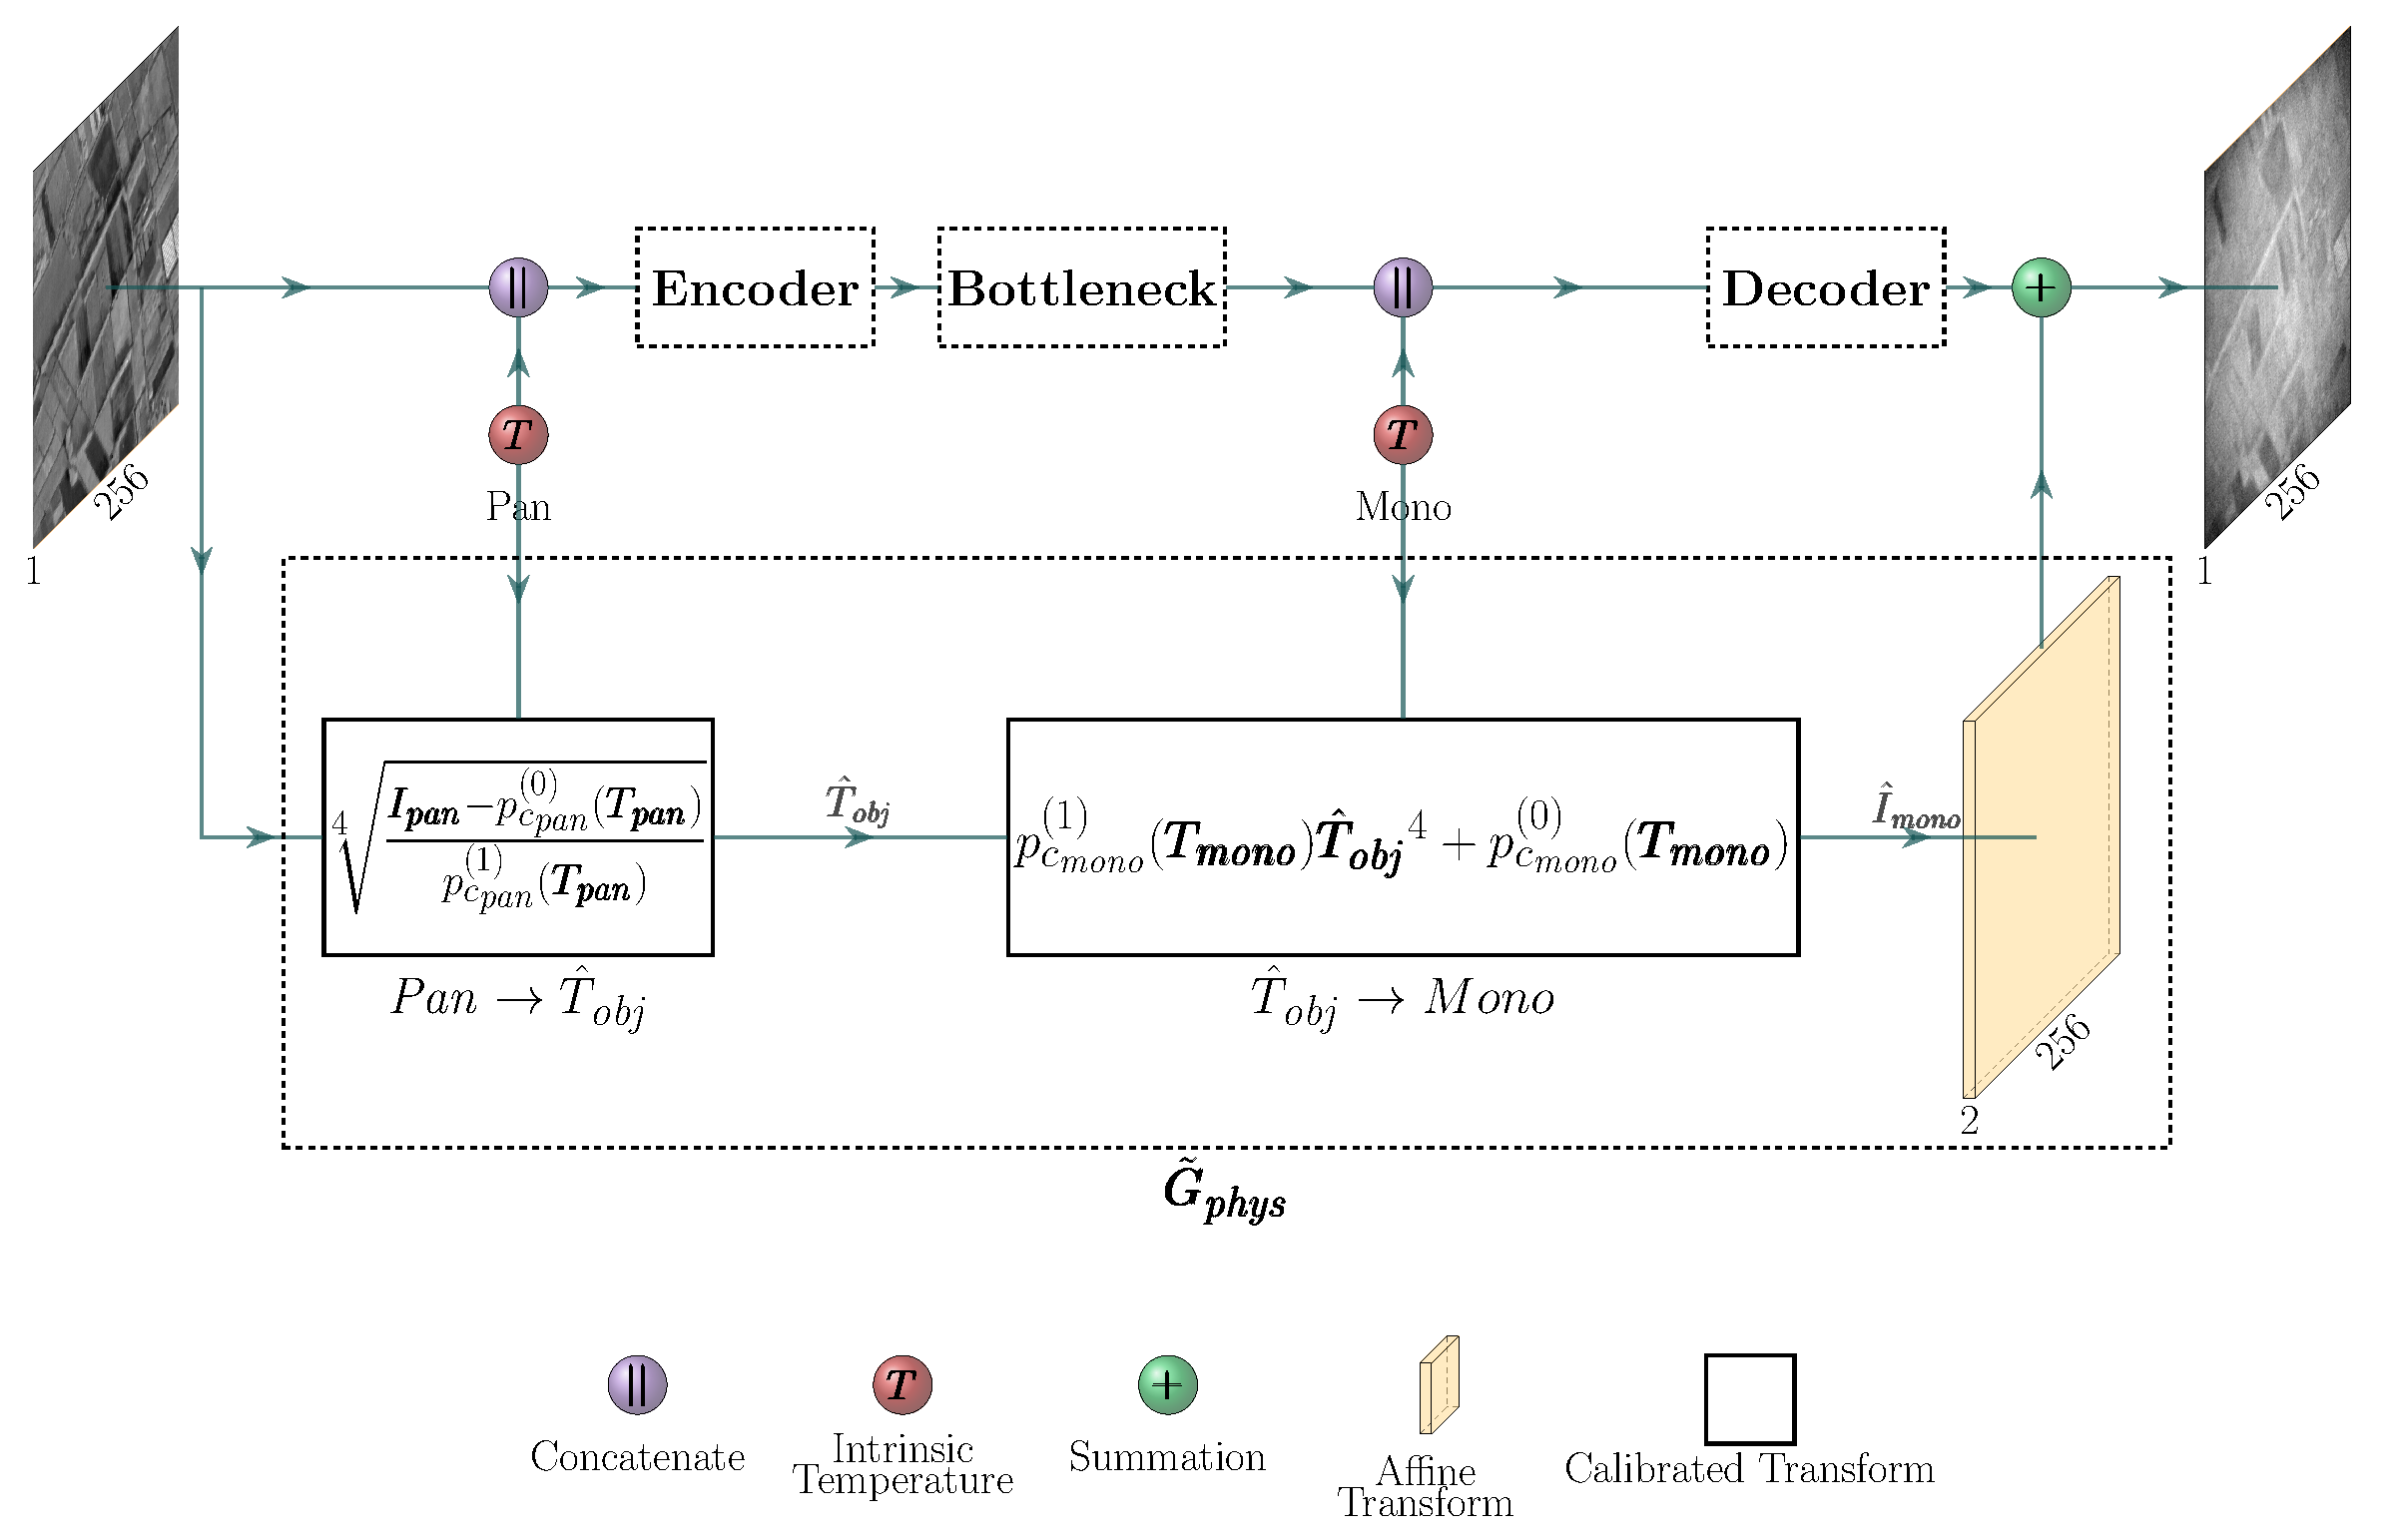
\includegraphics[width=\linewidth]{../figs/network/src/petit.pdf}
        \end{figure}  
        The physical estimator is used to produce a raw approximation of the desired output, leaving the deep estimator with the task of predicting the finer residual details.
    
    \end{itemize}
  
  \end{alertblock}

\end{column}

\separatorcolumn


% --------------------- 3rd column ---------------------
\begin{column}{\colwidth}

  \begin{block}{Quantitative Results}

    \begin{table}
    %   \centering
      \begin{tabular}{| c  c  c  c || c  c |}
          \multicolumn{4}{c}{Configuration} & \multicolumn{2}{c}{FID} \\
          \hline
          Backbone & Int & Phys & Caption & Mean & Std\\
          \hline   
          \multirow{4}{6em}{\centering CycleGan}  & \xmark & \xmark & Baseline    & 51.05             & 9.82\\      
                                                  & \xmark & \cmark &             & 35.54             & 3.72\\ 
                                                  & \cmark & \xmark &             & 50.17             & 8.89\\
                                                  & \cmark & \cmark & PETIT       & \textbf{33.8}     & \textbf{1.23}\\
          \hline
          \multirow{4}{6em}{\centering CUT}       & \xmark & \xmark & Baseline    & 38.43             & 1.52\\
                                                  & \xmark & \cmark &             & 29.85             & \textbf{0.99}\\
                                                  & \cmark & \xmark &             & 48.88             & 1.46\\
                                                  & \cmark & \cmark & PETIT       & \textbf{27.35}    & 1.01\\
          \hline
      \end{tabular}
    \end{table}  
  \end{block}

  \begin{block}{Qualitative Results}
    In accordance with the quantitative results, the monochromatic outputs produced by PETIT seem to be of superior quality compared to all other configurations.
    Generally speaking, PETIT's outputs incur less spurious artifacts and exhibit stronger fidelity to real monochromatic modality.
      \begin{figure}
        % 1st Row
        \centering
        \begin{subfigure}[b]{0.19\textwidth}
            \centering
            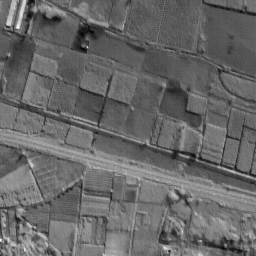
\includegraphics[width=\textwidth]{../figs/outputs/pan/71.png}
        \end{subfigure}
        \hfill
        \begin{subfigure}[b]{0.19\textwidth}
            \centering
            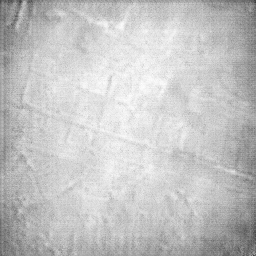
\includegraphics[width=\textwidth]{../figs/outputs/cycleGan/71.png}
        \end{subfigure}
        \hfill
        \begin{subfigure}[b]{0.19\textwidth}
            \centering
            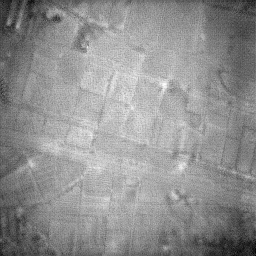
\includegraphics[width=\textwidth]{../figs/outputs/cut/71.png}
        \end{subfigure}
        \hfill
        \begin{subfigure}[b]{0.19\textwidth}
            \centering
            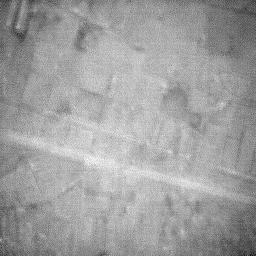
\includegraphics[width=\textwidth]{../figs/outputs/petit/71.png}
        \end{subfigure}
        \hfill
        \begin{subfigure}[b]{0.19\textwidth}
            \centering
            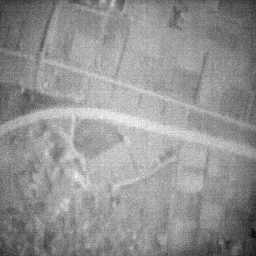
\includegraphics[width=\textwidth]{../figs/outputs/mono/605.png}
        \end{subfigure}      
        
        % 2nd Row
        \centering
        \begin{subfigure}[b]{0.19\textwidth}
            \centering
            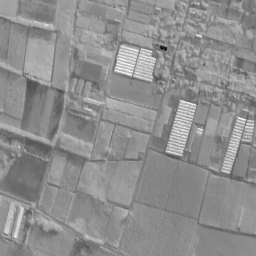
\includegraphics[width=\textwidth]{../figs/outputs/pan/24.png}
        \end{subfigure}
        \hfill
        \begin{subfigure}[b]{0.19\textwidth}
            \centering
            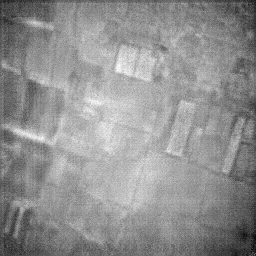
\includegraphics[width=\textwidth]{../figs/outputs/cycleGan/24.png}
        \end{subfigure}
        \hfill
        \begin{subfigure}[b]{0.19\textwidth}
            \centering
            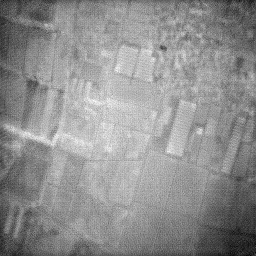
\includegraphics[width=\textwidth]{../figs/outputs/cut/24.png}
        \end{subfigure}
        \hfill
        \begin{subfigure}[b]{0.19\textwidth}
            \centering
            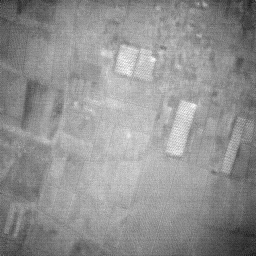
\includegraphics[width=\textwidth]{../figs/outputs/petit/24.png}
        \end{subfigure}
        \hfill
        \begin{subfigure}[b]{0.19\textwidth}
            \centering
            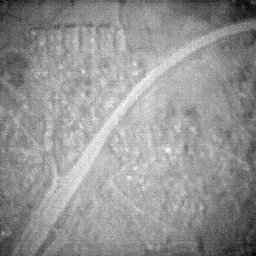
\includegraphics[width=\textwidth]{../figs/outputs/mono/508.png}
        \end{subfigure}    
        
        % 3rd Row
        \centering
        \begin{subfigure}[b]{0.19\textwidth}
            \centering
            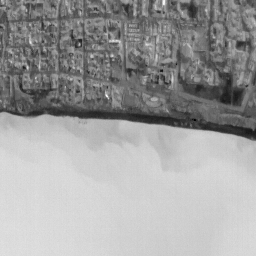
\includegraphics[width=\textwidth]{../figs/outputs/pan/28.png}
            \subcaption{Pan (input)}
            \label{fig:pan}
        \end{subfigure}
        \hfill
        \begin{subfigure}[b]{0.19\textwidth}
            \centering
            
\includegraphics[width=\textwidth]{../figs/outputs/cycleGan/28.png}
            \subcaption{CycleGAN}
            \label{fig:cycleGan}
        \end{subfigure}
        \hfill
        \begin{subfigure}[b]{0.19\textwidth}
            \centering
            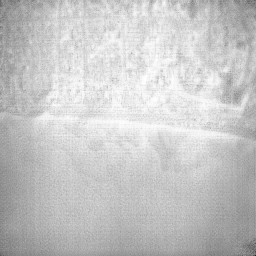
\includegraphics[width=\textwidth]{../figs/outputs/cut/28.png}
            \subcaption{CUT}
            \label{fig:cut}
        \end{subfigure}
        \hfill
        \begin{subfigure}[b]{0.19\textwidth}
            \centering
            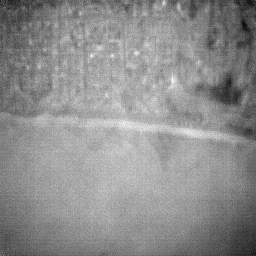
\includegraphics[width=\textwidth]{../figs/outputs/petit/28.png}
            \subcaption{PETIT}
            \label{fig:petit}
        \end{subfigure}
        \hfill
        \begin{subfigure}[b]{0.19\textwidth}
            \centering
            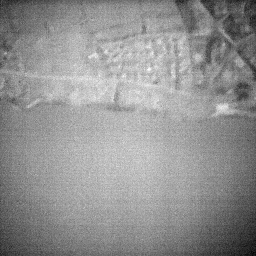
\includegraphics[width=\textwidth]{../figs/outputs/mono/994.png}
            \subcaption{Mono (ref)}
            \label{fig:mono}
        \end{subfigure}
      \end{figure}
  \end{block}

  \begin{block}{Conclusions}
    \begin{itemize}
      \item Physical modeling is beneficial for thermal UI2I translation. 
      \item PETIT beats deep SOTA UI2I models both quantitatively (by $\approx 50\%$!) and qualitatively.
      \item Fidelity of generated monochromatic images is good enough for synthesizing an artificial multispectral dataset.
    \end{itemize}      
  \end{block}

  \begin{block}{References}

    % \nocite{*}
    \footnotesize{\bibliographystyle{plain}\bibliography{../bib}}

  \end{block}

\end{column}

\separatorcolumn
\end{columns}
\end{frame}

\end{document}
